
\documentclass[16pt,a4paper]{article}
\usepackage[utf8]{inputenc}
\usepackage{amsmath}
\usepackage{amsfonts}
\usepackage{amssymb}
\usepackage{amsthm}

\usepackage{hyperref}

\hypersetup{
    colorlinks=true,
    linkcolor=blue,
    filecolor=magenta,      
    urlcolor=cyan,
    pdftitle={Sharelatex Example},
    bookmarks=true,
    pdfpagemode=FullScreen,
}



\usepackage[many]{tcolorbox}
\tcbuselibrary{skins,breakable}


\newtcbtheorem{defn}{Definition}{
    width=\textwidth,
    colback=white!20,
    colframe=orange,
    colbacktitle=orange,
    fonttitle=\bfseries,
    sharp corners,
    boxrule=1pt,
    breakable,
    enhanced,
    boxed title style={sharp corners},
    attach boxed title to top left
}{def}


\newtcbtheorem{axm}{Axiom}{
    width=\textwidth,
    colback=white!20,
    colframe=black,
    colbacktitle=black,
    fonttitle=\bfseries,
    sharp corners,
    boxrule=1pt,
    breakable,
    enhanced jigsaw,
    boxed title style={sharp corners},
    attach boxed title to top left
}{axm}


\newtcbtheorem{thm}{Theorem}{
    width=\textwidth,
    colback=blue!10,
    colframe=blue,
    colbacktitle=blue,
    fonttitle=\bfseries,
    sharp corners,
    boxrule=1pt,
    breakable,
    enhanced,
    boxed title style={sharp corners},
    attach boxed title to top left
}{thm}




\newtcbtheorem{coll}{Corollary}{
    width=\textwidth,
    colback=white!20,
    colframe=red,
    colbacktitle=red,
    fonttitle=\bfseries,
    sharp corners,
    boxrule=1pt,
    breakable,
    enhanced,
    boxed title style={sharp corners},
    attach boxed title to top left
}{coll}













\usepackage{setspace}
\setstretch{1.7}
\usepackage{graphicx}
\usepackage[left=2cm,right=2cm,top=2cm,bottom=2cm]{geometry}
\usepackage{tikz}
\usetikzlibrary{shapes, arrows, fit}
\usetikzlibrary{positioning}

\usepackage{listings}
\usepackage{color}
\definecolor{dkgreen}{rgb}{0,0.6,0}
\definecolor{gray}{rgb}{0.5,0.5,0.5}
\definecolor{mauve}{rgb}{0.58,0,0.82}

\definecolor{deepblue}{rgb}{0,0,0.5}
\definecolor{deepred}{rgb}{0.6,0,0}
\definecolor{deepgreen}{rgb}{0,0.5,0}
\lstset{frame=tb,
  language=python,
  aboveskip=2mm,
  belowskip=2mm,
  showstringspaces=false,
  columns=flexible,
  basicstyle={\linespread{0.9}\small	tfamily},
  numbers=none,
  numberstyle=	iny\color{gray},
  keywordstyle=\color{blue},
  commentstyle=\color{dkgreen},
  stringstyle=\color{deepred},
  breaklines=true,
  breakatwhitespace=true,
  tabsize=4
}
\let\oldemptyset\emptyset
\let\emptyset\varnothing

\theoremstyle{definition}
\newtheorem{definition}{Definition}[section]

\newtheorem{theorem}{Theorem}[section]
\newtheorem{corollary}{Corollary}[theorem]
\newtheorem{lemma}[theorem]{Lemma}


\newcommand{\OR}{\vee}

\newcommand{\AND}{\wedge}
\newcommand{\ord}{\preceq}


\author{Thaqib Mo.}
\title{Math 145}
\begin{document}

\maketitle
\tableofcontents
\newpage
\section{Axioms of Existence and Exensionality}

\begin{axm}{Axiom of Existence}{Axiom1} There is a set containing no elements. For this set set $A$ the statement $X\in A$ is false for all sets $X$.
\end{axm}

\begin{axm}{Axiom of Extensionality}{Axiom2}
If two sets have the same elements then they are equal. In other words for sets $X,Y$ if $\forall x \in X : x\in Y$ and $\forall y\in Y : y\in X$ then $X=Y$. 
\end{axm}
This axiom useful in proving uniqueness of sets. A theorem that can be proved using these 2 axioms is:
\begin{thm}{Unique Empty set}{}
There is a unique set containing no elements. (Denoted by ($\emptyset$))
\end{thm}
\begin{proof}
The axiom of existence tells that a set with no elements exists. Assume we have 2 sets $A_1$ and $A_2$, each with no elements.  The statement $\forall a \in A_1 \Rightarrow a \in A_2$ is true (\textit{vacuously}). So each element of $A_1$ is an element of $A_2$, As $A_2$ is also empty. Similar argument follows. Therefore by \textit{axiom 2 (Exensionality)} $A_1 = A_2$. Therefore the empty set is unique. 
\end{proof}
\section{Comprehension}
This axioms captures the intuition that we should be able to define a set with certain properties without getting into \textit{Russell's paradox. } \\
\textbf{Russell's paradox}
Let us define a set $S$ with the following property:
\[S = \{X \; | \; X\notin X\}\]
This set is a set of sets that are not elements of themselves. The paradox arises when we ask $S\in S\;?$.\linebreak 
If $S\in S$ by definition of$S$ we have $S\notin S$ which is a contradiction. But now that we have $S\notin S$ then  by definition of $S$ we must have $S\in S$. This leads to a paradox.  The figure below shows the paradox. 

\begin{center}
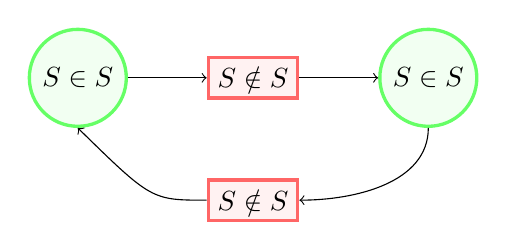
\begin{tikzpicture}[
roundnode/.style={circle, draw=green!60, fill=green!5, very thick, minimum size=7mm},
squarednode/.style={rectangle, draw=red!60, fill=red!5, very thick, minimum size=5mm},
]
%Nodes
\node[squarednode]      (maintopic)                              {$S\notin S$};
\node[roundnode]        (uppercircle)       [left=of maintopic] {$S\in S$};
\node[roundnode]      (rightsquare)       [right=of maintopic] {$S\in S$};
\node[squarednode]        (lowercircle)       [below=of maintopic] {$S\notin S$};

%Lines
\draw[->] (uppercircle.east) -- (maintopic.west);
\draw[->] (maintopic.east) -- (rightsquare.west);
\draw[->] (rightsquare.south) .. controls +(down:7mm) and +(right:7mm) .. (lowercircle.east);
\draw[->] (lowercircle.west) .. controls +(left:7mm) .. (uppercircle.south);
\end{tikzpicture}
\end{center}
The way around such a paradox is to define a set only when the sets come from a set already known to exist.
 \newpage

\begin{axm}{Axiom Schema of Comprehension}{Axiom3}
\label{Axiom3}
 Let $P(X)$ be a property of sets. For any set $A$, there is a set $B$ defined by the property  that $X\in B$ if and only if $X\in A$ and the statement $P(X)$ is true for all $X$.
 \end{axm}
Once we show that the set $B$ defined by the property $P(X)$ and set $A$ is unique. We can use the set builder notation to denote this set. The set $B$ in the \textit{axiom schema } will be written as
\[\{X\in A : P(X)\}\]


\begin{thm}{Uniqueness of set in Axiom Schema of Comprehension}{}
$\;$\\
For every set $A$ and property $P(X)$ of sets, the set $B$ defined by $A$ and $P(X)$ in (Axiom 3) is \textit{unique}. 
\end{thm}
\begin{proof}
By  \hyperref[Axiom3]{Axiom 3} we know that such a set exists. We need to prove uniqueness. Let $B_1$ and $B_2$ be 2 sets defined by the property that set $X$ is in these sets if and only if $X\in A$ and $P(X)$ is true. \\
So according to the definition any $X\in B_1$ also implies $X\in B_2$ by axiom of Exensionality we have $B_1 = B_2$. So the set $B$ given the axiom schema of comprehension is \textit{unique}. 
\end{proof}

\section{Pair, Union and Power Set}

\begin{axm}{Axiom of Pair}{}
 Given sets $A$ and $B$, there is a set $C$ whose elements are exactly $A$ and $B$. In other words we have $X\in C$ if and only if $X=A$ or $X=B$. 
\end{axm}
We can also show this set $C$ is unique by axiom of Exensionality. 
\begin{proof}
Let sets $C_1$ and $C_2$ be defined as $X\in C_1, C_2$ if and only if $X = A$ or $X=B$ for sets $A,B$. By definition we have,  for each $X\in C_1$ we have $X\in C_2$. Then by axiom of Exensionality we have $C_1 = C_2$
\end{proof}
We will use the notation $\{A,B\}$ for the set containing $A,B$ and in case $A=B$ we write $\{A\}$\\
The next axiom allows us to create larger sets from smaller ones.\\
 
 \newpage

 \begin{axm}{Axiom of Union}{}
 For any set $S$ there exists a set $U$ such that for any set $X$, $X\in U$ if and only if $X\in A$ for some $A\in S$. \end{axm}
Using this axiom we being with a set $S$ and use it to construct $U$, which will represent the union of all elements in $S$ (each element of $S$ is a set). A set belongs to the union $U$ exactly when it belongs to some member of $S$. \\
We can use Axiom of Extensionality to show that $U$ is unique for a given set $S$. The notation used for this is:
 \[\bigcup S\]
Represents the union of all elements of $S$. For example $\bigcup \{\emptyset, \{\emptyset\}\} = \{\emptyset\}$. As our definition states $x\in U$ if and only if $x\in A$ for some $A\in S$. We use the notation $A\cup B$ to represent $\bigcup\{A,B\}$

\begin{axm}{Axiom of power set}{}
For any set $A$, there exists a set $\mathcal{P}$, such that for any set $X, \; X\in \mathcal{P}$ if and only if $X\subseteq A$. 
\end{axm}
We can show the uniqueness using another axioms. The notation $\mathcal{P}(A)$ is used to denote the power set of $A$.  
Examples $\mathcal{P}(\{x_1, x_2\}) = \{\emptyset, \{x_1\}, \{x_2\}, \{x_1, x_2\}\}$. So in general for any set $A$ and the empty set $\emptyset$ are both subsets of $A$ so both are in $\mathcal{P(}A)$. \\


\textbf{Set Constructions}
Some of the common set constructions using axioms are:
\begin{itemize}
\item[\#] $A\cap B$, This can be constructed using \hyperref[Axiom3]{Axiom 3}. We define it as following: 
\[A\cap B = \{x\in A : x\in B\}\]
\item[\#] $A\setminus B$, This can also be constructed using axiom of comprehension.  
\[A\setminus B = \{x\in A : x \notin B\}\]
\end{itemize}

\newpage
\section{Natural Numbers and Successors}
We define natural numbers by the following property, every natural number $n$ is a set with exactly $n$ elements. As $\varnothing$ has no elements, it forces us to choose $0 = \varnothing$.\\
For sets with one element, all these sets have a single element: $\{\emptyset\}$, $\{\{\emptyset, \{\emptyset\}\}\}$, and $\{\{\emptyset\}\}$. More generally, for any set $x$, the set $\{x\}$ has one element. 
\\
One natural way to proceed is to define natural numbers based on the previously defined natural numbers. So $1 = \{0\}$, and $2 = \{1,0\}$ and so on. This leads to the recursive definition of a natural number $n$:
\[n = \{0,1,2, \ldots n-1\}\].\\
Another way to define a number $n+1$ (given numbers until $n$ are defined) is
\[n+1 = n \cup \{n\}\] 
Since the elements of $n+1$ are exactly the elements of $\{n\}$ and $n$ itself. 

\begin{defn}{Successor}{}
For any set $x$, the \textit{successor} of $x$ is the set $S(x) = x\cup \{x\}$
\end{defn}
So the natural numbers are what we get by applying successor to the empty set a finite number of times. 
\subsection{Inductive Sets and the Axiom of Infinity}
until now we do not have a way of explicitly defining the natural numbers based on the axioms we have so far. For this we need to define \textit{inductive set}
\begin{defn}{Inductive set}{}
A set $I$ is called \textit{inductive} if it has the following properties:
\begin{enumerate}
\item $0\in I$. 
\item if $n \in I$, then $S(n) \in I$
\end{enumerate}
\end{defn}

\newpage

\begin{axm}{Axiom of infinity}{} An inductive set exists. \end{axm}


Using this definition we can build $\mathbb{N}$. We let $\mathcal{I}$ to be the set said to exist by axiom of infinity, and use axiom of comprehension we have:
\[\mathbb{N} = \{x\in \mathcal{I} : x\in I \text{ for all inductive sets } I\}\]
\begin{thm}{}{}
$\mathbb{N}$ is \textit{inductive}
\end{thm}

\begin{proof}
We to justify the 2 properties of inductive sets. First, $0\in \mathbb{N}$, for every inductive set $I$ $0\in I$ by definition. Now assume that an element $n\in \mathbb{N}$, then by definition we have $n \in I$, for each such set $I$ we know that $n+1 \in I$. As $n+1$ belongs to every inductive set, hence it belongs to $\mathbb{N}$ as well.  
\end{proof}
To complete the construction of natural numbers we define a way to order the natural numbers. 
\begin{defn}{Ordering on $\mathbb{N}$}{}
Let $m,n \in \mathbb{N}$. We say that $m < n $ if $m \in n$
\end{defn}





\section{Ordered Pairs, Relations, and Cartesian Products}
\subsection{Ordered Pairs}
An ordered paid $(x,y)$ as the name suggest is ordered unlike sets. So an ordered paid $(x,y) \neq (y,x)$ the ordering of the elements matter. We can only have 2 ordered pairs equal $(x,y) = (x^\prime, y^\prime) \iff x = x^\prime\quad y = y^\prime$. \\
\begin{defn}{Ordered pair}{}
Given any 2 sets $x$ and $y$, the \textit{ordered paid} $(x,y)$ is defined to be the set \[\{\{x\}, \{x,y\}\}\]
\end{defn}\newpage
\begin{thm}{Uniqueness of ordered pairs}{}
For any sets $x,y,x_1, y_1$ we have $(x,y) = (x_1, y_1)$ if and only if $x = x_1$ and $y = y_1$. 
\end{thm}
\begin{proof}
($\Leftarrow$)\\
Assume $x = x_1$ and $y = y_1$
Then we have:
\begin{align*}
(x,y) = \{\{x\}, \{x,y\}\}\\
= \{\{x_1\}, \{x_1,y_1\}\}\\
= (x_1, y_1)
\end{align*}
($\Rightarrow$)
Now assume that $(x,y) = (x_1, y_1)$ due to the assumption we have
\[\{\{x\}, \{x,y\}\} = \{\{x_1\}, \{x_1,y_1\}\}\]
By axiom of Extensionality, 2 sets are equal if and only if they have the same elements. 
\begin{itemize}
\item Case 1: $x = y$
Then we have $\{\{x\}, \{x,y\}\} =  \{\{x\}\}$ by the above equality we must have $\{x\} = \{x_1\} \iff x = x_1$, and $\{x_1, y_1\} = \{x\}$ this is true if and only if $x = x_1$ and $x = y_1  = y$. There we have established $x = x_1$ and $y = y_1$
\item Case 2: $x \neq y$
Given the equality above $\{x,y\} = \{x_1\}$ is impossible then we must have $\{x,y\} = \{x_1, y_1\}$. Then it must be the case that $\{x\} = \{x_1\} \iff x = x_1$. 
\[\{x,y\} = \{x_1, y_1\} = \{x,y_1\}\]
Then we must have $y_1 = y$ this completes the proof. 
\end{itemize}
\end{proof}


\newpage
\subsection{Cartesian Products}
Informally the product of 2 sets $X\times Y$ is the collection of all ordered pairs. With first coordinate from $X$ and second from $Y$. In order to construct this product we need to supply a set with all elements of $X\times Y$. This can be defined as
\[X\times Y = \{w\in Z : w = (x,y) \text{ for some } x\in X, y\in Y\}\]   
The problem is what is this set $Z$?\\
First we need a set that contains the elements of $X$ and $Y$ this can be done with axiom of union. By constructing $X\cup Y$. Certainly $\{x\}$ and $\{x,y\}$ are both subsets of $X\cup Y$. So the elements of the set $\{x, \{x,y\}\}$ can be taken to belong to the power set $\mathcal{P(}X\cup Y)$\\
Now we have $\{x\} \in $ $\mathcal{P(}X\cup Y)$ and $\{x,y\} \in\mathcal{P(}X\cup Y)$. but the set $\{x, \{x,y\}\}$ is not a subset of $X\times Y$ so we cannot take $ Z = \mathcal{P(}X\cup Y)$. \\
To get a set of \textit{subsets} of $\mathcal{P(}X\cup Y)$ we need to consider the power set of this set. We need an element of $\mathcal{P(}\mathcal{P(}X\cup Y))$. As $\{\{x\}, \{x,y\}\} \in \mathcal{P(}\mathcal{P(}X\cup Y))$. So we can take $Z = \mathcal{P(}\mathcal{P(}X\cup Y))$ The formal definition is :
\begin{defn}{Product of sets}{}
Given any two sets $X$ and $Y$ , the Cartesian product of $X$ and $Y$ is the set
\[X\times Y = \{w\in \mathcal{P(}\mathcal{P(}X\cup Y)) \;:\; w = (x,y) \text{ for some } x\in X, y\in Y\}\]
\end{defn}

\subsection{Relations and Functions}
\begin{defn}{Binary Relation}{}
Given 2 sets a $A$, $B$ \textit{binary} relation from $A$ to $B$ is a subset of $A\times B$. More generally a set $R$ is called a \textit{relation} if all the elements of $R$ are ordered pairs. Rather than writing $(x,y) \in R$ we write $xRy$.
\end{defn}
\begin{defn}{Function}{}
A \textit{function} is a relation such if $(a,b_1)$ and $(a, b_2)$ in $f$ then we must have $b_1 = b_2$. If $(a,b)\in f$ we write $f(a) = b$ 
\end{defn}
A function from the set $A$ to $B$ is denoted by 
\[f:A \rightarrow B\]
\newpage
\subsection{Terminology Around Relations and Functions}
\begin{defn}{Domain and Range}{}
The \textbf{domain} of the relation $R$ is the set of all such $x$ such that $(x,y)\in R$ for some $y$. \\
The \textbf{range} of $R$ is the set of all such $y$ such that $(x,y)\in R$ for some $x$. 
We use ran$(R)$ and dom$(R)$ to denote the domain and range of $R$. 
The set ran$(R)\cup$dom$(R)$ is called the \textbf{\textit{\emph{field}}} of $R$.  
\end{defn}
All these definitions also apply to functions. 
\begin{defn}{Image, Inverse Image}{}
Let $R$ be a binary relation. The \textit{image} of set $A$ under $R$ is the set
\[R(A) = \{b\in \text{ran}(R) : (a,b) \in R \text{ for some } a\in A\}\]
Similarly given set $B$ the \textit{inverse image} of $B$ under $R$ is defined as
\[R^{-1} (B) = \{a\in \text{dom$R$} : (a,b)\in R \text{ for some $a\in A$}\}\]
\end{defn}
Given 2 relations their composition $R_2\circ R_1$ is defined as:
\[R_2 \circ R_1 = \{z\in \text{ dom$(R_2)\times$ ran$(R_1)$}\} : z = (a,c) \text{ such that $\exists b (a,b) \in R_1$ and $(b,c)\in R_2$}\}\]

\section{Invertibility, Injectivity, and Surjectivity}
A function is called Injective if for all $x_1, x_2 \in $dom$f$ such that $x_1 \neq x_2$. We have $f(x_1) \neq f(x_2)$. \\

If a function from $A$ to $B$ is called Surjective (onto) if ran$(f) = B$. In other words, for each $b\in B$ there exits $a\in A$ such that $f(a) = b$. \\

A function is called a bijection if it is both injective and surjective. 
\begin{figure}[hbpt]
\center
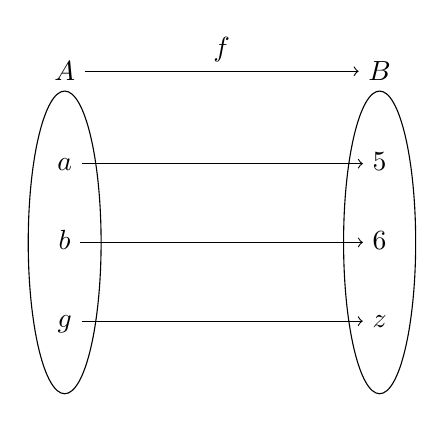
\begin{tikzpicture}[scale=2]
    \foreach[count=\i] \lseti/\lsetmi in {A/{$a$,$b$,$g$},B/{5,6,$z$}} {
        \begin{scope}[local bounding box=\lseti, x=2cm, y=0.5cm]
        \foreach[count=\j] \lj in \lsetmi {
            \node[minimum width=1em,anchor=base,text height=1.4ex,text
            depth=0.25ex] (n-\j-\lseti) 
            at (\i,-\j) {\lj};
        }
        \end{scope}
        \node[ellipse, draw, fit=(\lseti), 
        label={[name=l-\lseti]above:$\lseti$}] {};
    }
    \draw[->] (n-1-A) -- (n-1-B);
    \draw[->] (n-2-A) -- (n-2-B);
    \draw[->] (n-3-A) -- (n-3-B);
    \draw[->] (l-A) -- node[above]{$f$}(l-B);
\end{tikzpicture}
\end{figure}



\newpage

\section{Equivalence Relations}

\begin{defn}{Equivalence relation}{}
Let $R$ be be a binary relation on set $A$.  We say that 
\begin{itemize}
\item $R$ is \textit{reflexive} if , for all $a\in R$, we have $aRa$
\item $R$ is \textit{symmetric} if , for all $a,b \in A$  if $aRb$ then $bRa$
\item $R$ is \textit{transitive} if , for all $a,b,c \in A$ if $aRb$ and $bRc$ then $aRc$. 
\item $R$ is an equivalence relation if $R$ is reflexive, symmetric and transitive. 
\end{itemize}
\end{defn}

\subsection{Equivalence Classes}
\begin{defn}{Equivalence Class}{}
Suppose that $E$ is an equivalence relation on some set $A$. Given an element $a\in A$ the equivalence class of $a$ modulo $E$ is the set
\[[a]_E = \{x\in A : aEx\}\]
\end{defn}
So a equivalence relation splits up a set $A$ into smaller equivalence classes.  For any 2 elements in $A$ their equivalence classes are identical or they are disjoint. 
\begin{thm}{}{}
Let $E$ be an equivalence relation on set $A$. 
\begin{itemize}
\item[(1)] We have $aEb$ if and only if $[a] = [b]$
\item[(2)] We have $(a,b) \notin E$ if and only if $[a]\cap [b] = \varnothing$
\end{itemize}
\end{thm}

\begin{proof}
Assume that $aEb$. We have to prove that $[a] = [b]$. \\
Let $x\in [a]$ by definition we have $aEx$, since $E$ is symmetric and we know $aEb$ then $bEa$ as well. As $E$ is transitive and we have $bEa$ and $aEx$ this implies $bEx$. So we get $x\in [b]$ showing $[b] \subset [a]$ a symmetric argument for $[a] \subset [b]$ follows. Proving that $[a] = [b]$ is $aEb$. \\
 Next, assume $[a] = [b]$. Since $E$ is reflexive we know that $bEb$ so we have $b\in [b]$ but we have $[b] = [a]$ then we get $b\in [a]$ by definition we get $aEb$. 
 
 
We can prove $(2)$ if we have $[a] \cap [b] = \varnothing$ then $[a] \neq [b]$ because both $[a]$ and $[b]$ are non empty sets. On the other hand assume $[a] \cap [b] \neq \varnothing$. Then there is some $x \in [a] \cap [b]$ so we have $x \in [a]$ and $x\in [b]$. That is by definition $aEx$ and $bEx$ using the property of equivalence relations we can get to $aEb$. By part (1) we have $[a] = [b]$. 
\end{proof}




\newpage
\section{Partitions}
\begin{defn}{Partitions}{}
Given any set $A$, a \textit{partition} $\mathcal{P}$ of $A$ is a collection of  non empty sets with the properties:
\begin{itemize}
\item[(1)] For any two distinct sets $P_1, P_2 \in \mathcal{P}$, we have $P_1 \cap P_2 = \varnothing$
\item[(2)] $\bigcup \mathcal{P} = A$
\end{itemize}{} 
\end{defn}
Theorem 5 essentially shows that a every equivalence relation on $A$ gives us  a set $A$ gives us a partition of that set. We have the notation $A/E$ for the set $\{[a]_E : a \in A\}$. 
\begin{figure}[hbpt]
\centering
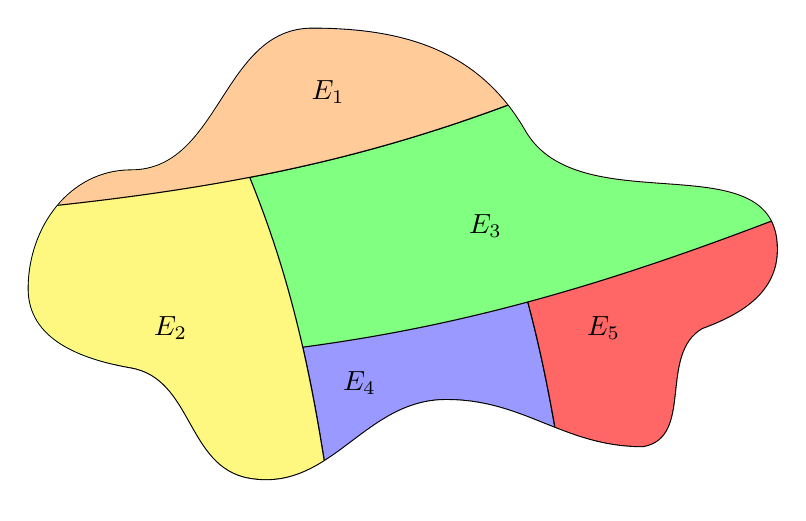
\begin{tikzpicture}
\path
  coordinate (aux0) at (0,1.5)
  coordinate (aux1) at (0,3.5)
  coordinate (aux2) at (10,3.5)
  coordinate (aux3) at (9,6)
  coordinate (aux4) at (4,0)
  coordinate (aux5) at (7,0)
  coordinate (aux6) at (2,6)
  coordinate (aux7) at (5,6)
  coordinate (esp1) at (0.2,2.5)
  coordinate (esp2) at (1.5,1.5)
  coordinate (esp3) at (3,0.1)
  coordinate (esp4) at (5.5,1.1)
  coordinate (esp5) at (8,0.5)
  coordinate (esp6) at (8.75,2)
  coordinate (esp7) at (9.7,3)
  coordinate (esp8) at (6.5,4.5)
  coordinate (esp9) at (3.8,5.8)
  coordinate (esp10) at (1.5,4)
  ;
\draw[line width=0.8pt]
  (esp1) to[out=-90,in=170]
  (esp2) to[out=-10,in=170]
  (esp3) to[out=-10,in=180]
  (esp4) to[out=0,in=180]
  (esp5) to[out=10,in=-150]
  (esp6) to[out=20,in=-90]
  (esp7) to[out=90,in=-60]
  (esp8) to[out=120,in=0]
  (esp9) to[out=180,in=0]
  (esp10) to[out=180,in=90]
  cycle;    
\clip
  (esp1) to[out=-90,in=170]
  (esp2) to[out=-10,in=170]
  (esp3) to[out=-10,in=180]
  (esp4) to[out=0,in=180]
  (esp5) to[out=10,in=-150]
  (esp6) to[out=20,in=-90]
  (esp7) to[out=90,in=-60]
  (esp8) to[out=120,in=0]
  (esp9) to[out=180,in=0]
  (esp10) to[out=180,in=90]
  cycle;    
\filldraw[fill=blue!40]
  (aux4) to[bend right=10]
  (aux6) --
  (aux7) to[bend left=10]
  (aux5) -- cycle;
\filldraw[fill=red!60]
  (aux5) to[bend right=10]
  (aux7) --
  (10,6) --
  (10,0) -- cycle;
\filldraw[fill=green!50]
  (aux0) -- 
  (aux1) to[bend right=10]
  (aux3) --
  (10,6) -- 
  (aux2) to[bend left=10] cycle;
\filldraw[fill=yellow!50]
  (0,0) -- 
  (aux4) to[bend right=10]
  (aux6) --
  (0,6) -- 
  (0,0) -- cycle;
\filldraw[fill=orange!40]
  (0,6) -- 
  (aux1) to[bend right=10]
  (aux3) --
  (0,6) -- cycle;
\node at (4,5) {$E_1$};  
\node at (2,2) {$E_2$};  
\node at (6,3.3) {$E_3$};  
\node at (4.4,1.3) {$E_4$};  
\node at (7.5,2) {$E_5$};  
\end{tikzpicture}


\end{figure}
\begin{thm}{}{}
Let $E$ be a equivalence relation on $A$. Then $A/E$ is a partition of $A$. 
\end{thm}
\begin{proof}
Every equivalence class $[a]$ is non empty as we must have $a \in [a]$. According to \textbf{lemma 1.1} if 2 equivalence classes are not equal they are disjoint. Which verifies condition (1) for partitions. Condition (2) follows from the fact that every $a\in A$ belongs to its equivalence class $[a]$, so the union of all equivalence classes $[a]$ is the set whole set $A$
\end{proof}
Therefore \emph{every equivalence relation gives rise to a partition.} We can also show that the converse is true: That every partition can be used to define an equivalence relation on that set. 
\newpage
\begin{thm}{}{}
Let $A$ be a set , and let $\mathcal{P}$ be a partition on that set. We define a relation $E$ on $A$ by stating $a_1 E a_2$ if there is some $P \in \mathcal{P}$ such that $a_1 \in P$ and $a_2 \in P$. Then $E$ is an equivalence relation on $A$. 
\end{thm}
\begin{proof}
$\;$\\
\begin{itemize}
\item \textbf{Reflexivity} Let $a\in A$ be arbitrary. Since $\mathcal{P}$ is a partition, there is some $P \in \mathcal{P}$ containing $a$. So clearly $a\in P$ and $a\in P$ then we have $aEa$ for every $a\in A$. 

\item \textbf{Symmetry} Suppose we have $a_1, a_2 \in A$ such that $a_1 E a_2$. There there is some $P \in \mathcal{P}$ such that $a_1 \in P$ and $a_2 \in P$. Symmetrically we also have $a_2 \in P$ and $a_1 \in P$ leading to $a_2 E a_1$

\item \textbf{Transitivity} Suppose we have $a_1, a_2, a_3 \in A$ such that $a_1Ea_2$ and $a_2Ea_3$. Then for some $P_1\in\mathcal{P}$ we have $a_1 \in P_1$ and $a_2 \in P_1$, and also for some $P_2 \in \mathcal{P}$ we have $a_2 \in P_2$ and $a_3 \in P_2$. Since $\mathcal{P}$ is a partition if $P_1$ and $P_2$ were distinct we would have $P_1 \cap P_2 = \varnothing$. But this is not the case as $a_2$ is in both sets. Therefore we have $P_1 = P_2$. So $a_1$ and $a_3$ are in the same $P_1 \in \mathcal{P}$ leading to $a_1 E a_3$ 

\end{itemize}
\end{proof} 
Therefore, we see that this correspondence runs both ways: every equivalence relation gives a partition, and every partition gives an equivalence relation.


\begin{defn}{}{}
Let $A$ be a set and $E$ be an equivalence relation on $A$.  A set $X$ is called the \textit{set of representatives} for $E$ if $X$ contains exactly one element from each equivalence class. \\
In other words, for each $[a] \in A/E$ we have $X\cup [a] = \{\alpha\}$ for some $\alpha \in [a]$. 
\end{defn}
These equivalence classes can be visualized using this figure:  
\begin{center}
\begin{figure}[hbpt]
\center
\begin{tikzpicture}[scale = 2]

\node (a) at (1,3) {$a$};
\node (b) at (0,2) {$b$};
\node (c) at (3,2.5) {$c$};
\node (d) at (3,1.5) {$d$};
\node (e) at (1,1) {$e$};
\node (f) at (2,2) {$f$};
\node (g) at (1,0) {$g$};
\node (h) at (2,0) {$h$};

\draw
 (a) edge (b) edge (e) edge (f)
 (b) edge (e) edge (f)
 (e) edge (f)

 (c) edge (d)
 (g) edge (h)
;

\node[draw,fit=(a)(b)(e)(f)] {};
\node[draw,fit=(c)(d)] {};
\node[draw,fit=(g)(h)] {};

\end{tikzpicture}

\end{figure}
\end{center}


\newpage
\section{Order Relations}
\begin{defn}{Antisymmetric Relation}{}
Let $R$ be a binary relation on set $A$. We say that $R$ if, whenever we have $a,b \in A$ such that $aRb$ and $bRa$, it follows that $a=b$. A relation $\ord$ is an order relation on $A$ if if it is reflexive , \textit{antisymmetric}, and transitive.
\end{defn}
\subsection{Chains and Extremal Elements}
\begin{defn}{Total ordering}{}
If $\ord$ is a partial ordering on set $A$ we say that 2 elements $a,b \in A$ are comparable if either $a\ord b$ or $b \ord a$. A partial order in which every pair of elements is comparable is called a \textit{total ordering} or \textit{linear ordering}. \\
\end{defn}
{\color{red} Example} The relation $\leq$ on $\mathbb{Z}$ is a total ordering as every pair $a,b \in \mathbb{Z}$ are comparable. 

Another important notion which comes is the notion of a \textit{chain}:
\begin{defn}{Chain}{}
If $\ord$ is a partial order on set $A$, a subset $C$ of $A$ is called a \textit{chain} if every pair of $C$ are comparable. In particular, if $\ord$ is a total order on $A$ then $A$ itself is a chain in $A$. 
\end{defn}

Because not every element of a set must be comparable we have to be careful in distinguishing the greatest and the least elements of of a given set. The distinction is given by the following definitions. 
\begin{defn}{Maximal, minimal, greatest, least elements}{}
Let $A$ be a set with partial order relation $\ord$. Given a subset $B$ of $A$ we say that 
\begin{itemize}
\item An element $b\in B$ is the \textbf{least element} of $B$ if we have $b\ord b^\prime$ for all $b^\prime \in B$. Similarly, an element is the \textbf{greatest element} if $b^\prime \ord b$ for all $b^\prime\in B$. 

\item An element $b\in B$ is the \textbf{minimal element} of $B$ if there are no smaller elements, that is if $b^\prime \ord b$ \textbf{for some} $b^\prime \in B$ then $b = b^\prime$. Similarly an element is the \textbf{maximal element} if there are no larger elements, that is if $b \ord b^\prime$ \textbf{for some} $b^\prime \in B$ then $b^\prime = b$. 
\end{itemize}
\end{defn}

\newpage
\section{Bounds on Sets, Suprema, and Infima}
\begin{defn}{Bounds, Suprema, and Infima}{}
Suppose $A$ is a set with order relation $\ord$ and with a subset $B$. 
\begin{itemize}
\item An element $a\in A$ is a lower bound for $B$ if $a\ord b$ \textbf{for all} $b\in B$. Similarly $a\in A$ is a upper bound for $B$ if $b \ord a$ \textbf{for all} $b\in B$. 

\item An element $a\in A$ is the infimum (Greatest lower bound) of $B$ if $a$ is the greatest element of the set of al lower bounds for $B$. 

\item Am element $a\in A$ is the supremum (Least upper bound) of $B$ if $a$ is the least element of the set of all upper bounds for $B$. 
\\
If they exist, we use $sup\;B$ and $inf \;B$ to denote the supremum and infimum of a set $B$, respectively.
 
\end{itemize}
\end{defn}

\newpage



\section{Axiom of choice}

Suppose $\mathcal{C}$ is a non empty collection of sets then the Cartesian product of all sets in $\mathcal{C}$ is written as:

\[\prod\limits_{C\in \mathcal{C}} C\] 

If $\mathcal{C}$ is an infinite collection of sets then we need infinite ordered tuple of elements. Then we need a function $\alpha : \mathcal{C} \rightarrow \bigcup \mathcal{C}$. Then for each $C\in \mathcal{C}$ we have $\alpha(C) \in C$. The function $\alpha (C)$ should give the $C$-th coordinate of the infinite tuple. We can formally define this as:\\

\begin{defn}{Cartesian Product for infinite sets}{}
Let $\mathcal{C}$ denote a non empty collection of sets. The Cartesian product $\prod\limits_{C\in \mathcal{C}}C$  is the set of all functions $\alpha : \mathcal{C} \rightarrow \bigcup \mathcal{C}$  with the property $\alpha(C) \in C$.
\end{defn} 

We can use this definition to redefine the Cartesian product, even for finitely many sets. We can define an ordered pair $(a,b) \in A\times B$ as $(\alpha(A), \alpha(B))\in A\times B$. \\
The problem arises when for an infinite number of sets in $\mathcal{C}$ we cannot show (using the standard axioms of set theory) that:

\[\prod_{C\in \mathcal{C}}C \neq \varnothing\]
For this we need a new axiom. 

\begin{axm}{Axiom of Choice}{}
The Cartesian product of any non-empty collection of non-empty sets is
non-empty.
\end{axm}
This axiom is also equivalent to the existence of a choice function for every non-empty collection of set $\mathcal{C}$.   

\begin{figure}[hbtp]

\centering
\includegraphics[scale=1]{figs/fig0.png}
\end{figure}



\newpage

\section{Zorn's Lemma and the Well-Ordering Theorem}

Another statement about partially ordered set is logically equivalent to Axiom of choice. 


\begin{thm}{Zorn's Lemma}{}
Let $A$ be a partially ordered set with order relation $\preceq$. Suppose that every chain in $A$ has an upper bound in $A$, then $A$ has a maximal element. 
\end{thm}


A Corollary that follows from Zorn's Lemma is:

\begin{coll}{}{}
Suppose that $A$ is a partially ordered set with order relation $\preceq$ then every chain $\mathcal{C}$ in $A$ is contained in a maximal chain $\mathcal{M}$. 
\end{coll}
\begin{proof}
Let $\mathcal{C}$ be an arbitrary chain in $A$. Consider the set $\Gamma$ of all chains $\mathcal{C}$ in $A$. The subset relation $\subseteq$ relation on $\mathcal{P}(A)$ giving the order relation between elements of $\Gamma$. Now suppose we have a chain $\mathcal{D}$ in the ordered set $\Gamma$. We can show that $\mathcal{D}$ is an upper bound in $\gamma$
\\

If we define $\mathcal{C}_0 = \bigcup \mathcal{D}$, the union of all the, clearly for each $\mathcal{C}^\prime \in \mathcal{D}$ we have $C^\prime \subseteq \mathcal{C}_0$. Since $C_0$ contains every chain of $\mathcal{D}$, each of which contains $\mathcal{C}$ we know that $\mathcal{C}_0$ contains $\mathcal{C}$. Therefore $C_0$ is an upper bound on $\mathcal{D}$ by definition. If we can verify $C_0 \in \Gamma $ that means $C_0$ is a chain in $A$
\\

Suppose we have  $a_1, a_2 \in \mathcal{C}_0$. By construction each element of $a_1$ and $a_2$ belong to a chain in $\mathcal{D}$, so we can write $a_1 \in \mathcal{C}_1$ and $a_2 \in \mathcal{C}_2$. Since $\mathcal{D}$ is a chain with respect to the relation $\subseteq$, we can either have $\mathcal{C}_1\subseteq \mathcal{C}_2$ or we can have $\mathcal{C}_2\subseteq \mathcal{C}_1$. Without loss of generality we say $\mathcal{C}_1\subseteq \mathcal{C}_2$ . Thus both $a_1, a_2 \in C_2$. Since $\mathcal{C}_2$ is a chain, the elements in $\mathcal{C}_2$ are comparable with $\preceq$, this verifies that $\mathcal{C}_0$ is a chain in $A$, as $C_0 \in \Gamma$. 
\\

Now if we apply Zorns lemma to $\Gamma$ which is ordered by $\subseteq$, there is a chain $\mathcal{M} \in \Gamma$, maximal with respect to the containment relation $\subseteq$. This is a chain in $A$ with respect to the ordering $\preceq$, as it is maximal with with respect to $\subseteq$ all chains $\mathcal{C}$ of $A$ are contained in $\mathcal{M}$ and it is not properly contained in any chain.  


\end{proof}




\newpage
The well ordering theorem is another statement known to be equivalent to axiom of choice. We can define the WOP of $\mathbb{N}$ more generally. 
\begin{defn}{Well ordering}{}
Suppose $A$ is a set with order relation $\preceq$. The ordered set $A$ is said to be well ordered if every non empty subset of $A$ has a least element with respect to the relation $\preceq$
\end{defn}

This leads to the well ordering theorem:

\begin{thm}{Well-Ordering Theorem}{}
Every non empty set has a well ordering. 
\end{thm}

In other words, if $A$ is a non empty set then there is a an order relation $\preceq$ on $A$, such that $A$ is well ordered with respect to $\preceq$. This means that the set $\mathbb{R}$ has as well ordering, not with respect to the relation $\leq$ as this fails for any open interval in $\mathbb{R}$ but according to \textit{well ordering theorem} there exits a relation $\preceq$ on $\mathbb{R}$ on which every subset of $\mathbb{R}$ will have a least element with respect to $\preceq$ which is not the relation $\leq$. 
\\

The 3 statements Axiom of choice, Well-Ordering Theorem, Zorn's Lemma are all logically equivalent.    















































































































































































































































\end{document}
